\documentclass[12pt]{article}
\usepackage[utf8]{inputenc}
\usepackage[a4paper, total={6.5in, 8.5in}]{geometry}
\usepackage{authblk}
\usepackage{multirow}
\usepackage{graphicx}
\usepackage{amsmath}
\usepackage{biblatex}
\usepackage{rotating}
\usepackage{ragged2e}
\usepackage{multicol}
\usepackage{float}
\usepackage{algpseudocode}
\usepackage{enumitem}
\usepackage{caption}
\usepackage{subcaption}
\usepackage{hyperref}
\hypersetup{
    colorlinks=true,
    linkcolor=blue,
    }
\usepackage[label=corner]{karnaugh-map}
\usepackage[siunitx, RPvoltages]{circuitikz}
\usetikzlibrary{calc}
\usepackage{tikz}
\usetikzlibrary{positioning}

\title{CSE 306 \\
Computer Architecture Sessional \\
\vspace{10mm}
Assignment-1: 4-bit ALU Simulation \\
\vspace{20mm}
Section - A1 \\
Group - 01 \\
\vspace{15mm}
\RaggedRight
Members of the Group: \\
\normalsize	{
\begin{enumerate}[label=\roman*]
    \item 1905001 - Mohammad Sadat Hossain
    \item 1905002 - Nafis Tahmid
    \item 1905004 - Asif Azad
    \item 1905005 - Md. Ashrafur Rahman Khan
    \item 1905008 - Shattik Islam Rhythm
\end{enumerate}
}
}
\author{}
\date{}

\begin{document}

\maketitle

\newpage
\section{\large{Introduction}}
ALU, elaborated as Arithmetic and Logic Unit, is quite simply the mathematical brain of a computer. It is mainly a combinational digital circuit that performs arithmetic and bitwise and logical operations on integer binary numbers. Needless to say, it is a core building block of any computing unit, ranging from Central Processing Unit (CPU) to Graphics Processing Unit (GPU)s.\\
As the name suggests, an ALU comprises of two main units: Arithmetic Unit and Logic Unit. It supports a wide range of operations including arithmetic ones like addition, subtraction, increment, decrement, transfer, and logical ones like NOT, OR, XOR, AND etc. The control unit routes the source information from registers into ALU inputs. To select a particular operation, an ALU has some selection lines or bits. Decoding system allows to support $2^k$ different operations for $k$ selection lines or bits. In our implemented ALU, there are $3$ control selection inputs.\\
A parallel adder is the heart of the arithmetic part of the ALU.
Multiplexed inputs to the IC paves the way to achieve expected results for varieties of arithmetic operations. Besides, logical operations can be performed with their respective ICs, and in some efficient designs, a particular IC is used to do a different operation other than its intended one.\\
There are also 4 status outputs (flags) in our designed ALU. They are denoted by C(Carry Flag), Z(Zero Flag), V(Overflow Flag), S(Sign Flag). Their representations carry out the following meanings:
\begin{description}
 \item[CF:] CF is simply the $C_{out}$ of the adder used in the ALU. So, any carry out results in it being 1, otherwise it is set to 0. Logical operations cause it to be 0.
 \item[ZF:] If the last operation of the ALU yielded an output of 0, ZF is set, else it is 0.
 \item[VF:] If after any arithmetic operation, two positive numbers result in a negative output, or two negative numbers result in a positive output, that is an overflow and VF is set. After any logical operation, it is cleared.

 \begin{equation} \label{eq1}
\begin{split}
S_3 & = A_3 \oplus I_3 \oplus C_3\\
\implies C_3 & = S_3 \oplus A_3 \oplus I_3
\end{split}
\end{equation}
\begin{equation} \label{eq2}
    \begin{split}
        V & = C_3 \oplus C_{out}\\
    \end{split}
\end{equation}
Combining \ref{eq1} and \ref{eq2},\\
\begin{equation*}
    V = A_3 \oplus I_3 \oplus S_3 \oplus C_{out}\\
\end{equation*}

 Here, $I_3$ is either $B_3$ from input (MSB of $B$), or $c$ depending on selected operation, $S_3$ is the MSB of the adder output and $C_{out}$ is the output carry of the adder.
 \item[SF:] It reflects the output MSB.
\end{description}


\newpage
\section{\large{Problem Specification with Assigned Instructions}}
Design a 4-bit ALU with three selection bits cs0, cs1 and cs2 for performing the following operations:
\begin{table}[H]
    \centering
    \begin{tabular}{||c|c|c|l|l||}
    \hline
         \multicolumn{3}{||c|}{Control Signals} & \multirow{2}{*}{Functions} & \multirow{2}{*}{Description}\\
         \cline{1-3}
         cs2 & cs1 & cs0 & & \\
         \hline
         \hline
         0 & X & 0 & Add & $A + B$ \\
         0 & 0 & 1 & AND & $A \cap B$ \\
         0 & 1 & 1 & Transfer A & Output is A\\
         1 & 0 & 0 & Decrement A & $A - 1$\\
         1 & 0 & 1 & XOR & $A \oplus B$\\
         1 & 1 & X & Add with Carry & $A + B + 1$\\
         \hline
    \end{tabular}
    \caption{Problem Specification}
    \label{tab:Table1}
\end{table}
\vspace{15mm}

% \begin{figure}[H]
%     \centering
%     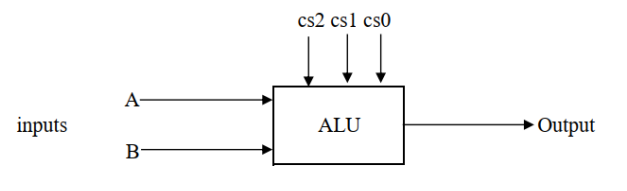
\includegraphics[width=0.8\textwidth]{alu_block_1.png}
%     \caption{4-bit ALU}
%     \label{fig:alu_block_1}
% \end{figure}

\begin{figure}[H]
\centering
\begin{tikzpicture}
    \node[draw, rectangle, minimum width=3.5cm, minimum height=2cm] (alu) at (0, 0){ALU};
    \draw[latex-] (alu.130) |- ++ (0, 1.5) node[above left=1.5cm and -1.35cm of alu] {cs2};
    \draw[latex-] (alu.90) |- ++ (0, 1.5) node[above left=1.5cm and -2.20cm of alu] {cs1};
    \draw[latex-] (alu.50) |- ++ (0, 1.5) node[above left=1.5cm and -3.10cm of alu] {cs0};
    \node at (-6, 0) {Input};
    \draw[latex-] (alu.165) -- ++ (-2, 0) node[pos=1.1] {A};
    \draw[latex-] (alu.195) -- ++ (-2, 0) node[pos=1.1] {B};
    \draw[-latex] (alu.east) -- ++ (2, 0) node[pos=1.45] {Output};
\end{tikzpicture}
    \vspace{5mm}
    \caption{4-bit ALU}
    \label{fig:alu_block_1}
\end{figure}



\newpage
\section{\large{Detailed Design Steps with K-maps}}

\subsection{Design Steps}
\begin{enumerate}
    \item The arithmetic unit computes 4 arithmetic operations (Add, Add with Carry, Transfer A and Decrement A) with the help of a 4-bit full adder and a multiplexer.

    \item For the adder, the first input $A$ is fixed; the second input is $B$ or $c$ which is selected by the multiplexer having $S_0$ selection bit. For Add and Add with Carry operations, $B$ is selected whereas for Transfer $A$ and Decrement $A$ operations, $c$ is selected. $c=0000$ for Transfer $A$ and $c=1111$ for Decrement $A$.

    \item In the arithmetic unit, the adder adds $A$, $B$ with $C_{in}=0$ and $C_{in}=1$ for Add, Add with Carry operations respectively. $c=0000, C_{in}=0$ for transfer operation, so adder outputs $A+0+0=A$. During decrement operation, $c=1111$, $C_{in}=0$ that is adder adds $1111$ to $A$ which is basically equivalent to $A-1+0=A-1$ in signed representation.

    \item The logical unit performs $2$ logical operations AND, XOR using $1$ AND IC, $1$ XOR IC and the output (AND, XOR) of the logical unit is selected by a multiplexer having selection bit $S_1$ ($0$ for XOR, $1$ for AND).

    \item A third multiplexer selects the final output of the ALU. For selection bit $S_2=0$, the output of the arithmetic unit is the final output and for $S_2=1$, the output of the logical unit is the final output.

    \item The overflow flag, VF and carry flag, CF is computed from the arithmetic unit. During logical operations, $C_{in}=0$ and $c=0000$ is selected as the second input of the adder. So there is no chance of overflow and carry keeping $VF=0, CF=0$ for logical operations.

    \item Zero flag, ZF is computed by adding the 4 output bits using 3 OR gates and then inverting $O_0 + O_1+O_2+O_3$ by 1 XOR gate($X\oplus1=\overline{X}$).

\end{enumerate}

\subsection{K-maps}
We will be following Table \ref{tab:truth_table} to construct the K-maps for intermediate selection bits.
\subsubsection{K-map for $S_0$}
$S_0$ is the selection bit for the multiplexer that selects the second input of the adder in the arithmetic unit. There are two alternatives for the second input of the adder $B$ or $c$. $B$ is the second user input which will be selected in case of add and add with carry operation. $c$ can be $1111$ or $0000$ and will be used respectively for decrement and transfer operations. ($c$ will also be used in case of logical operations to maintain the carry and overflow flags.)\\
\begin{center}
\begin{karnaugh-map}[2][4][1][$cs0$][$cs1$][$cs2$]
    \minterms{0, 2, 6, 7}
    \maxterms{1, 3, 4, 5}
    \implicant{0}{2}
    \implicant{6}{7}
\end{karnaugh-map}
\end{center}
So, there are four minterms. We will be using decoders (active low output) to implement the minterms.
\[ S_0 = D_0 + D_2 + D_6 + D_7 = \overline{\overline{D_0} . \overline{D_2}} +  \overline{\overline{D_6} . \overline{D_7}} \]

\subsubsection{K-map for $S_1$}
$S_1$ is the selection bit for the multiplexer which selects between XOR and AND operation inside logic unit.
\begin{center}
\begin{karnaugh-map}[2][4][1][$cs0$][$cs1$][$cs2$]
    \minterms{1}
    \maxterms{5}
    \terms{0, 2, 3, 4, 6, 7}{X}
    \implicant{5}{5}
\end{karnaugh-map}
\end{center}
We can easily express $S_1$ with only one minterm. But we will use the maxterm instead as our decoder is active low.
\[S_1 = \overline{D_5}\]

\subsubsection{K-map for $S_2$}
$S_2$ is the selection bit for the multiplexer that selects between the output of the arithmetic and logic unit which eventually is the ALU output.
\begin{center}
\begin{karnaugh-map}[2][4][1][$cs0$][$cs1$][$cs2$]
    \minterms{1, 5}
    \maxterms{0, 2, 3, 4, 6, 7}
    \implicantedge{1}{1}{5}{5}
\end{karnaugh-map}
\end{center}

We will do similar treatment as $S_0$.
\[S_2 = D_1 + D_5 = \overline{\overline{D_1} . \overline{D_5}}\]

\subsubsection{K-map for $C_{in}$}
It is the input carry bit of the adder used inside arithmetic unit. It will be $1$ only at the time of Add with carry operation. (At the time of logical operation, we will design the selection bits to select transfer operation in arithmetic unit to ensure the flags are in correct state. So, $C_{in}$ will be $0$ in those cases too.)
\begin{center}
\begin{karnaugh-map}[2][4][1][$cs0$][$cs1$][$cs2$]
    \minterms{6, 7}
    \maxterms{0, 1, 2, 3, 4, 5}
    \implicant{6}{7}
\end{karnaugh-map}
\end{center}
\[C_{in} =  D_6 + D_7 = \overline{\overline{D_6} . \overline{D_7}}\]

\subsubsection{K-map for $c$}
$c$ is the alternative input for the second input of the adder inside Arithmetic unit. it will be $1$ in case of decrement operator and $0$ in case of transfer operation. ($c$ will be input to all 4 bits of second input of the adder when selected.)
\begin{center}
\begin{karnaugh-map}[2][4][1][$cs0$][$cs1$][$cs2$]
    \minterms{4}
    \maxterms{1, 3, 5}
    \terms{0, 2, 6, 7}{X}
    \implicant{0}{4}
\end{karnaugh-map}
\end{center}
As there can be only one bit in the simplified expression, we do not need decoder output in this case.
\[c = \overline{cs0}\]

\newpage
\section{\large{Truth Table}}
For better interpretation of the variables used, refer to Figure \ref{fig:block_diagram}.
\begin{table}[H]
    \centering
    \begin{tabular}{|ccc|c|c|c|c|c|c|}
    \hline
         cs2 & cs1 & cs0 & Function & $c$ & $C_{in}$ & $S_0$ & $S_1$ & $S_2$  \\
         \hline
         0 & 0 & 0 & Add & X & 0 & 1 & X & 0  \\
         0 & 0 & 1 & AND & 0 & 0 & 0 & 1 & 1 \\
         0 & 1 & 0 & Add & X & 0 & 1 & X & 0 \\
         0 & 1 & 1 & Transfer A & 0 & 0 & 0 & X & 0 \\
         1 & 0 & 0 & Decrement A & 1 & 0 & 0 & X & 0 \\
         1 & 0 & 1 & XOR & 0 & 0 & 0 & 0 & 1 \\
         1 & 1 & 0 & Add with Carry & X & 1 & 1 & X & 0 \\
         1 & 1 & 1 & Add with Carry & X & 1 & 1 & X & 0 \\
         \hline
    \end{tabular}
    \caption{Truth Table for Intermediate I/0}
    \label{tab:truth_table}
\end{table}


\newpage
\section{\large{Block Diagram}}
\vspace{15mm}
\ctikzset{
    logic ports=ieee,
    logic ports/scale=1
}
\begin{figure}[h]
    \centering

\begin{circuitikz}
\tikzset{mux/.style={muxdemux,
 muxdemux def={Lh=5, NL=2, Rh=3,
 NB=1, w=2.5, square pins=1}}}


\tikzset{adder/.style={muxdemux,
 muxdemux def={Lh=6, NL=2, Rh=6, NT=1,
 NB=1, w=3, square pins=1}}}

\node[mux](mux1) at (0,0){MUX};
\draw (mux1.bpin 1) node[below]{$S_0$};
\draw (mux1.lpin 1) -- ++(-0.5, 0) node[left]{$ c $};
\draw (mux1.lpin 2) -- ++(-0.5, 0) node[left]{$ B $};
\draw (mux1.rpin 1) -- ++(0.4,0) node[above](d){$I$} -- ++(0.6,0) node[adder, anchor=lpin 2](adder){Adder};
\draw (adder.lpin 1) -- ++(-0.4,0) node[left](a1){$ A $};
\draw (adder.tpin 1) -- ++(0,3) node[left]{$ C_{out} $} -- ++(10.3,0) node[right]{$ \mathbf{C} $};
\draw (adder.bpin 1) -- ++(0,-1) node[below]{$ C_{in} $};
\draw (adder.rpin 1) -- ++(0.5, 0) node[below](e){$ E $} -- ++(0.5,0) node[mux, anchor=lpin 1](mux2){MUX};
\draw (mux2.lpin 2) -- ++(-0.5, 0) -- ++(0, -5) -- ++(-1,0) node[mux, anchor=rpin 1](mux3){MUX};
\draw (mux3.lpin 1) -- ++(-0.5, 0) node[xor port, anchor=out](xor){};
\draw (mux3.lpin 2) -- ++(-0.5, 0) node[and port, anchor=out](and){};
\draw (xor.in 1) --++(-0.5,0) node[left]{$ A $};
\draw (xor.in 2) --++(-0.5,0) node[left]{$ B $};
\draw (and.in 1) --++(-0.5,0) node[left]{$ A $};
\draw (and.in 2) --++(-0.5,0) node[left]{$ B $};
\draw (mux2.bpin 1) node[below]{$ S_2 $};
\draw (mux3.bpin 1) node[below]{$ S_1 $};
\draw (mux2.rpin 1) --++(0.7,0) coordinate(Y) --++(0,0) node[right]{$Y$};
\draw (Y) --++ (0, 0.2) coordinate(y)
          --++(0, 0.5) node[left](y0){\tiny $Y_0$};
\draw (y0) --++(0.5, 0) node[or port, number inputs=4, inner inputs=4, anchor=in 4](or){};
\draw (y) -- (y |- or.in 3) node[left]{\tiny $Y_1$} -- (or.in 3);
\draw (y) -- (y |- or.in 2) node[left]{\tiny $Y_2$} -- (or.in 2);
\draw (y) -- (y |- or.in 1) node[left](Y3){\tiny $Y_3$} -- (or.in 1);
\draw (or.out) --++(0.5,0) node[xor port, anchor=in 2](xor2){};
\draw (xor2.in 1) --++(-0.5,0) node[left]{$1$};
\draw (xor2.out) --++(0.5,0) node[right]{$\mathbf{Z}$};
\node[xor port, number inputs=4, inner inputs=4](xor3) at ($(xor2)+(0,3)$){};
\draw (xor3.in 4) -- (xor3.in 4 -| e) node[left](e3){\tiny $E_3$} -- (e);
\draw (xor3.in 3) -- (xor3.in 3 -| adder.tpin 1);
\draw (xor3.in 2) -- ($(xor3.in 2 -| a1)+(0.4,0)$) node[left](t1){\tiny $A_3$} -- ++(0,-3);
\draw (xor3.in 1) -- ($(xor3.in 1 -| d)+(0.65,0)$) node[left](t1){\tiny $I_3$} -- ++(0,-4.96);
\draw (or.in 1) --++(-0.1,0) --++(0,1.3) --++(5.5,0) node[right]{$\mathbf{S}$};
\draw (xor3.out) --++(0.5,0) node[right]{$\mathbf{V}$};

\end{circuitikz}
 \caption{Block Diagram of ALU}
    \label{fig:block_diagram}
\end{figure}

\section{\large{Complete Circuit Diagram}}

     \begin{figure}[H]
         \centering
         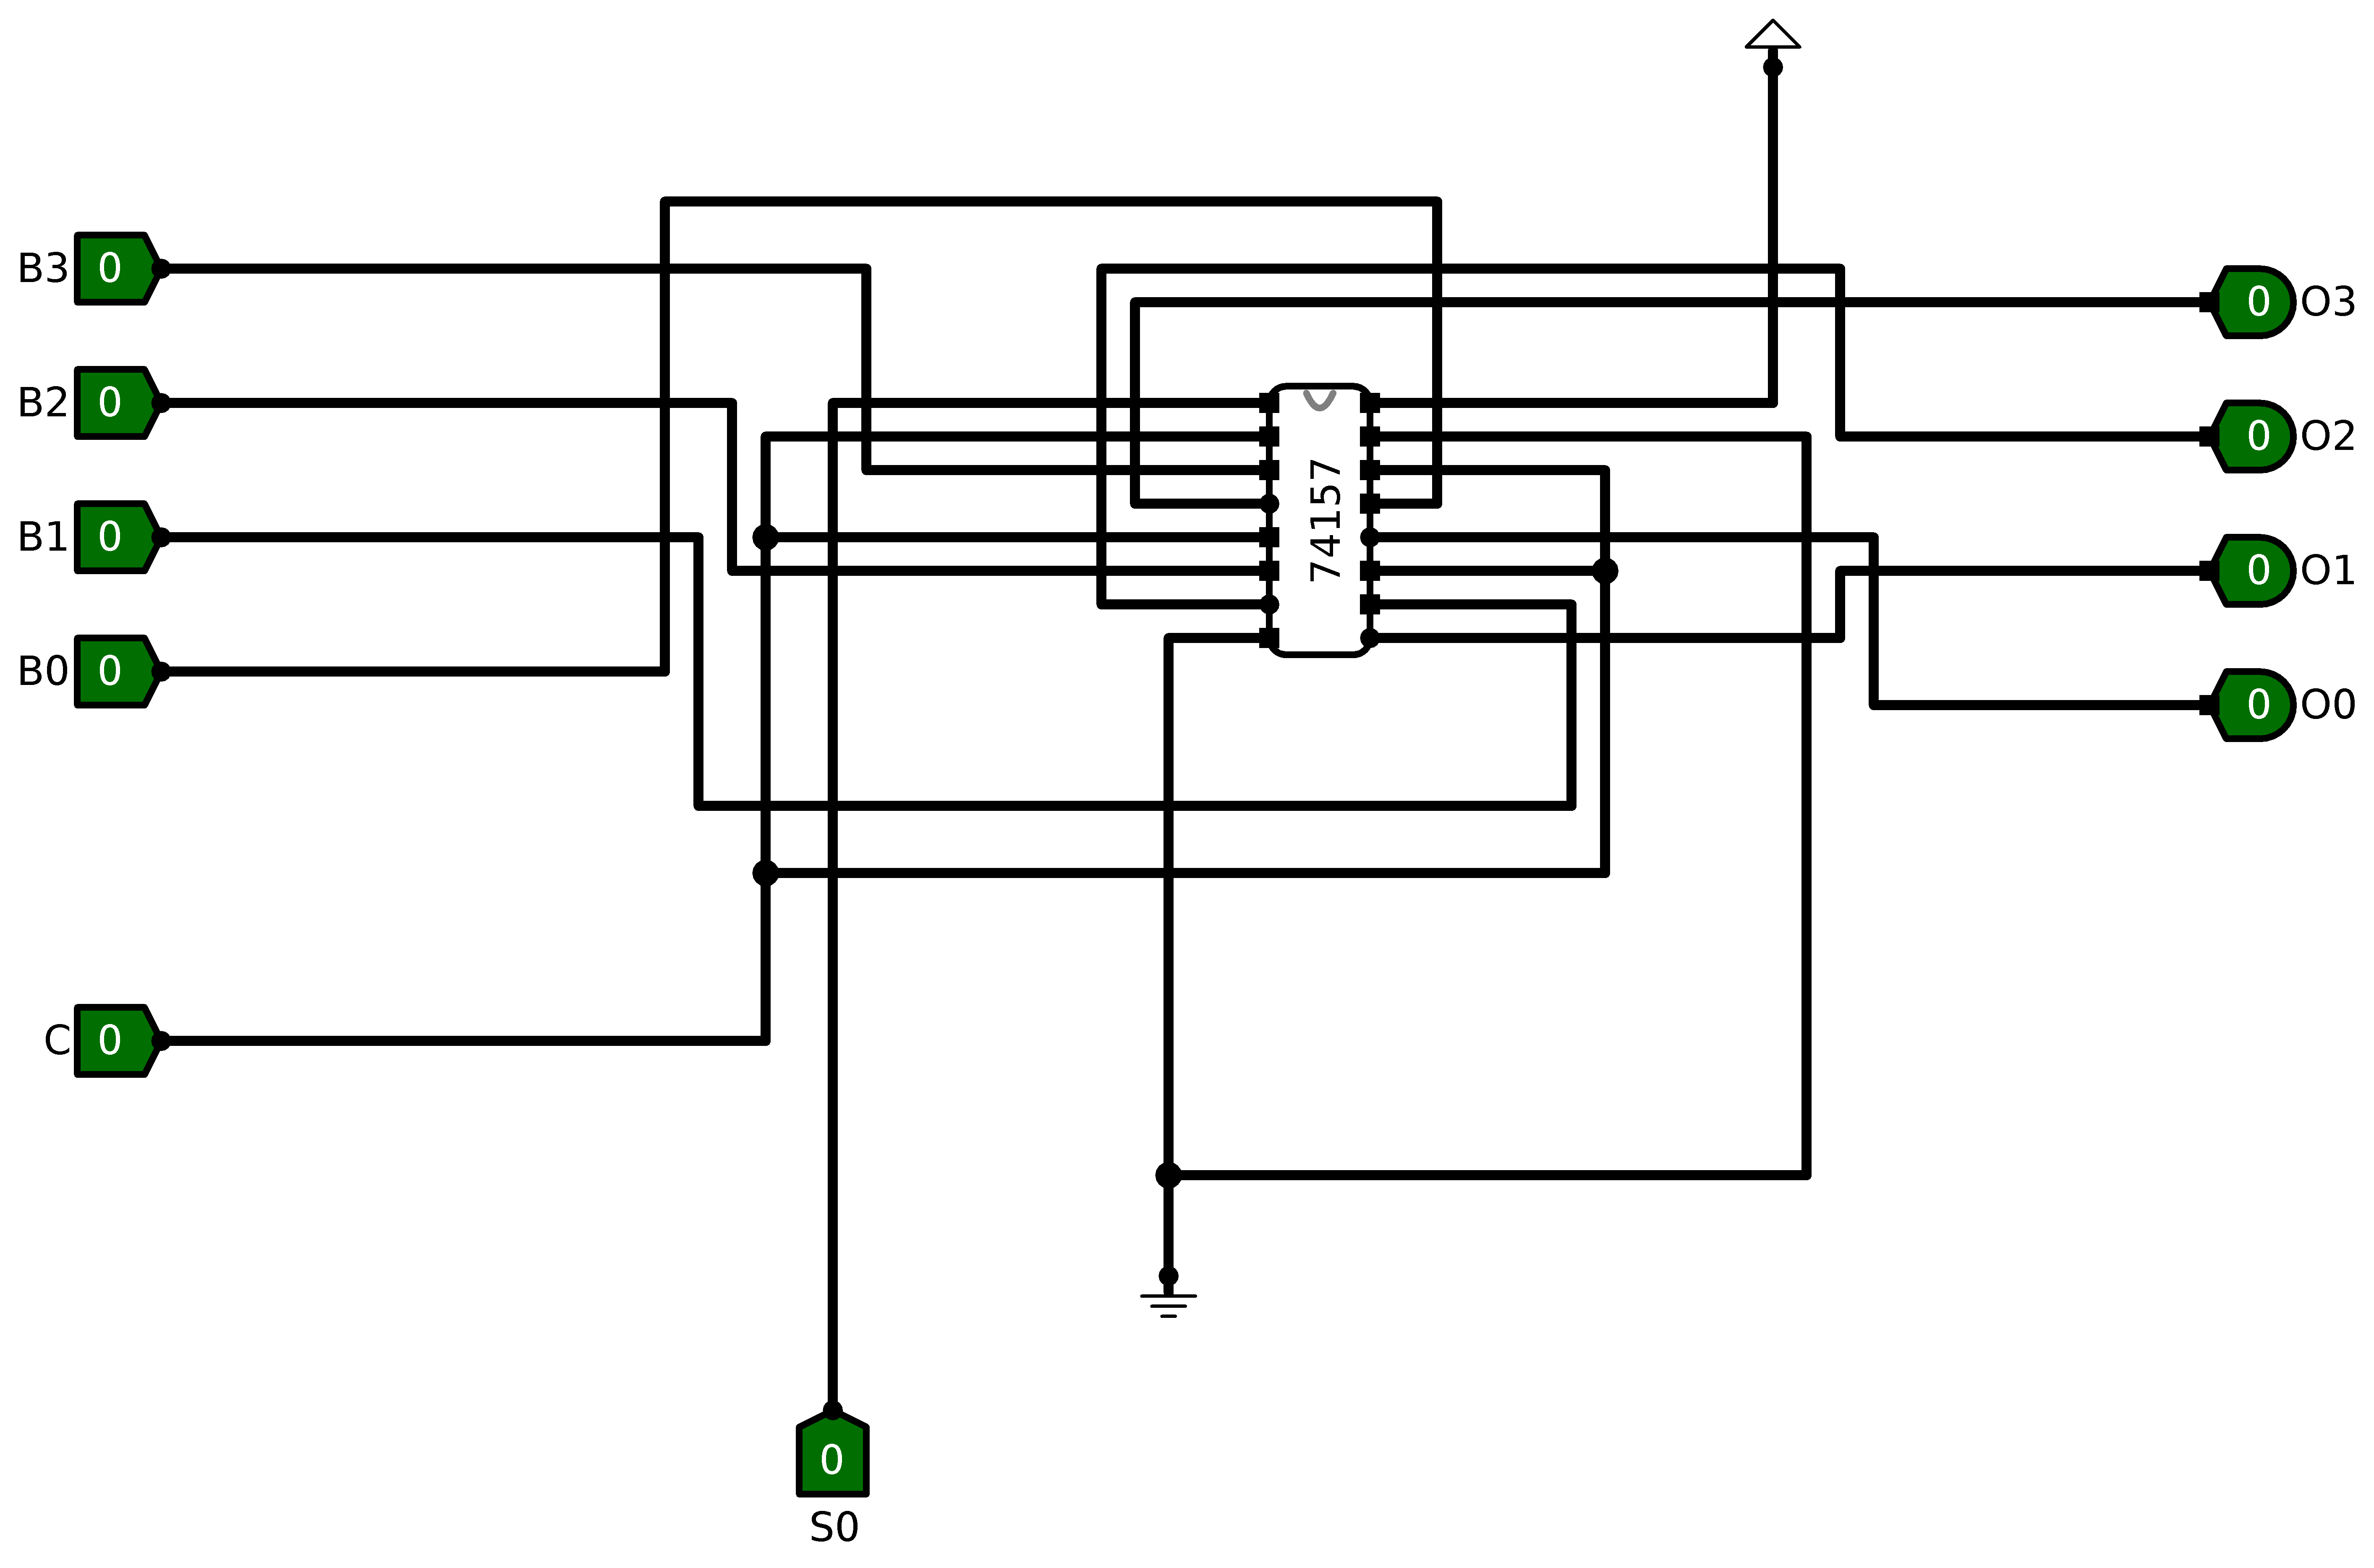
\includegraphics[width=0.8\textwidth]{Input for AU.png}
         \caption{Input Processing for Arithmetic Unit}
         \label{fig:alu_a}
     \end{figure}
     \begin{figure}[H]
         \centering
         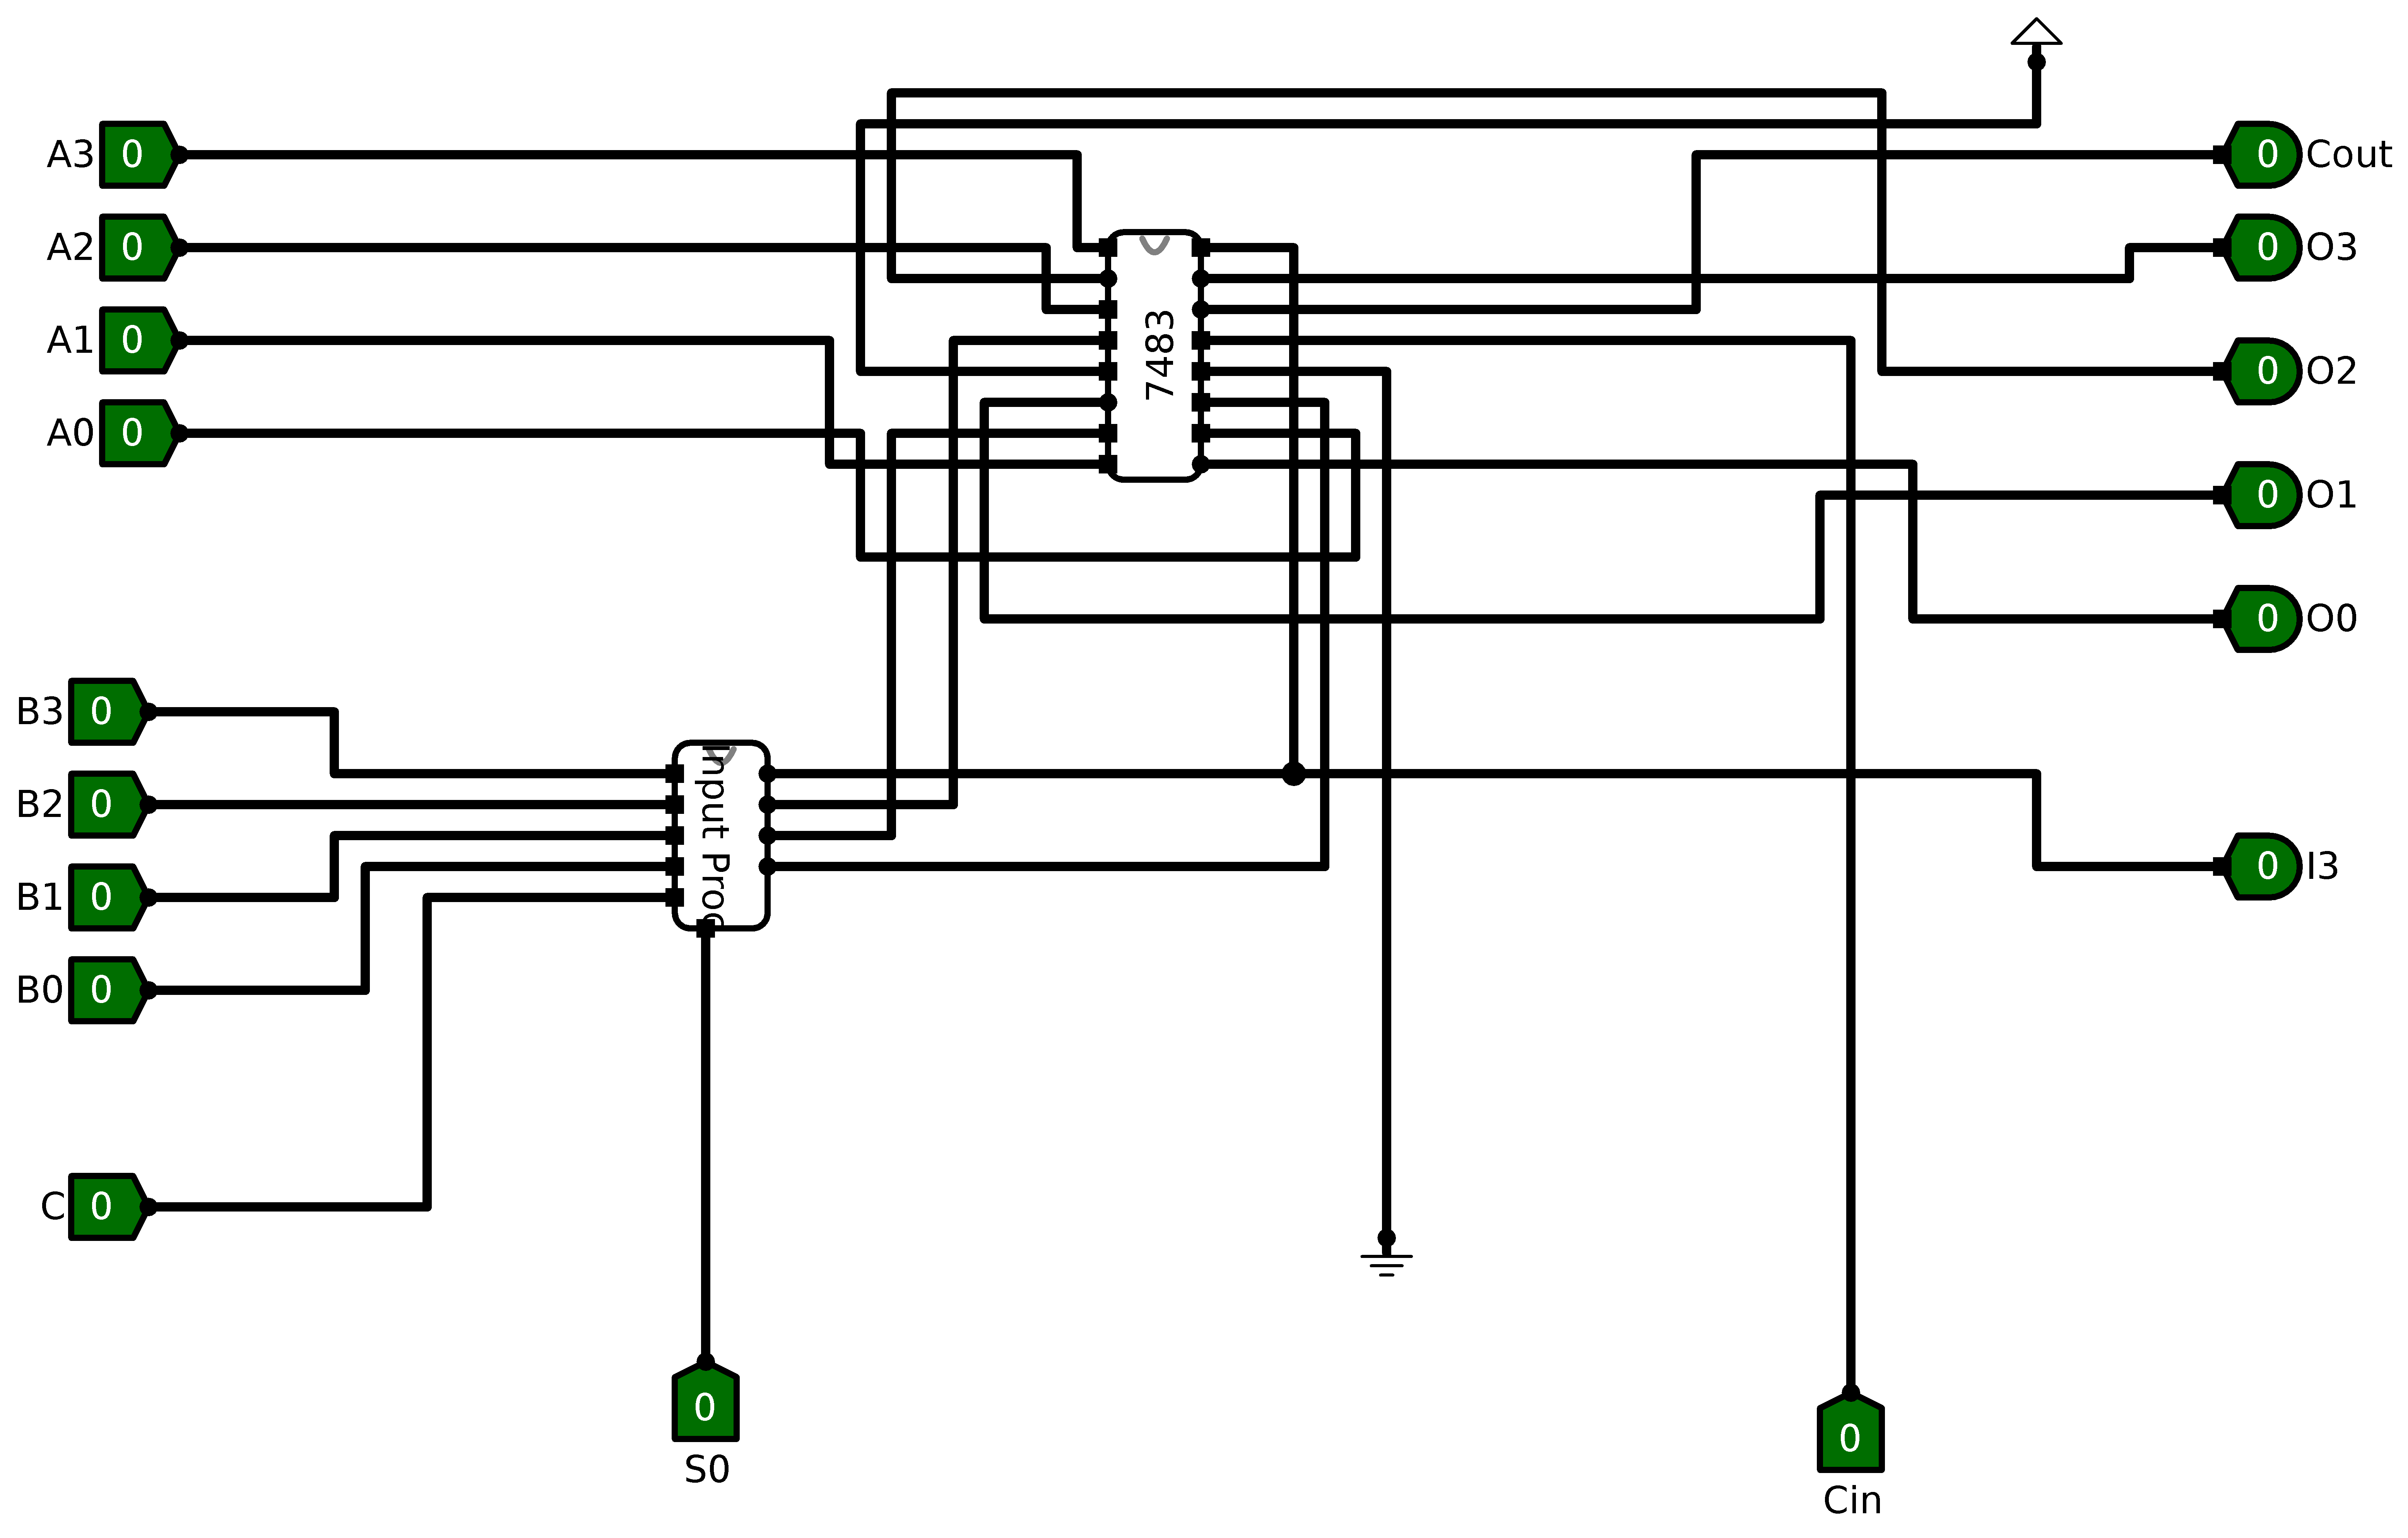
\includegraphics[width=0.8\textwidth]{Arithmetic Unit.png}
         \caption{Arithmetic Unit}
         \label{fig:alu_b}
     \end{figure}
     \begin{figure}[H]
         \centering
         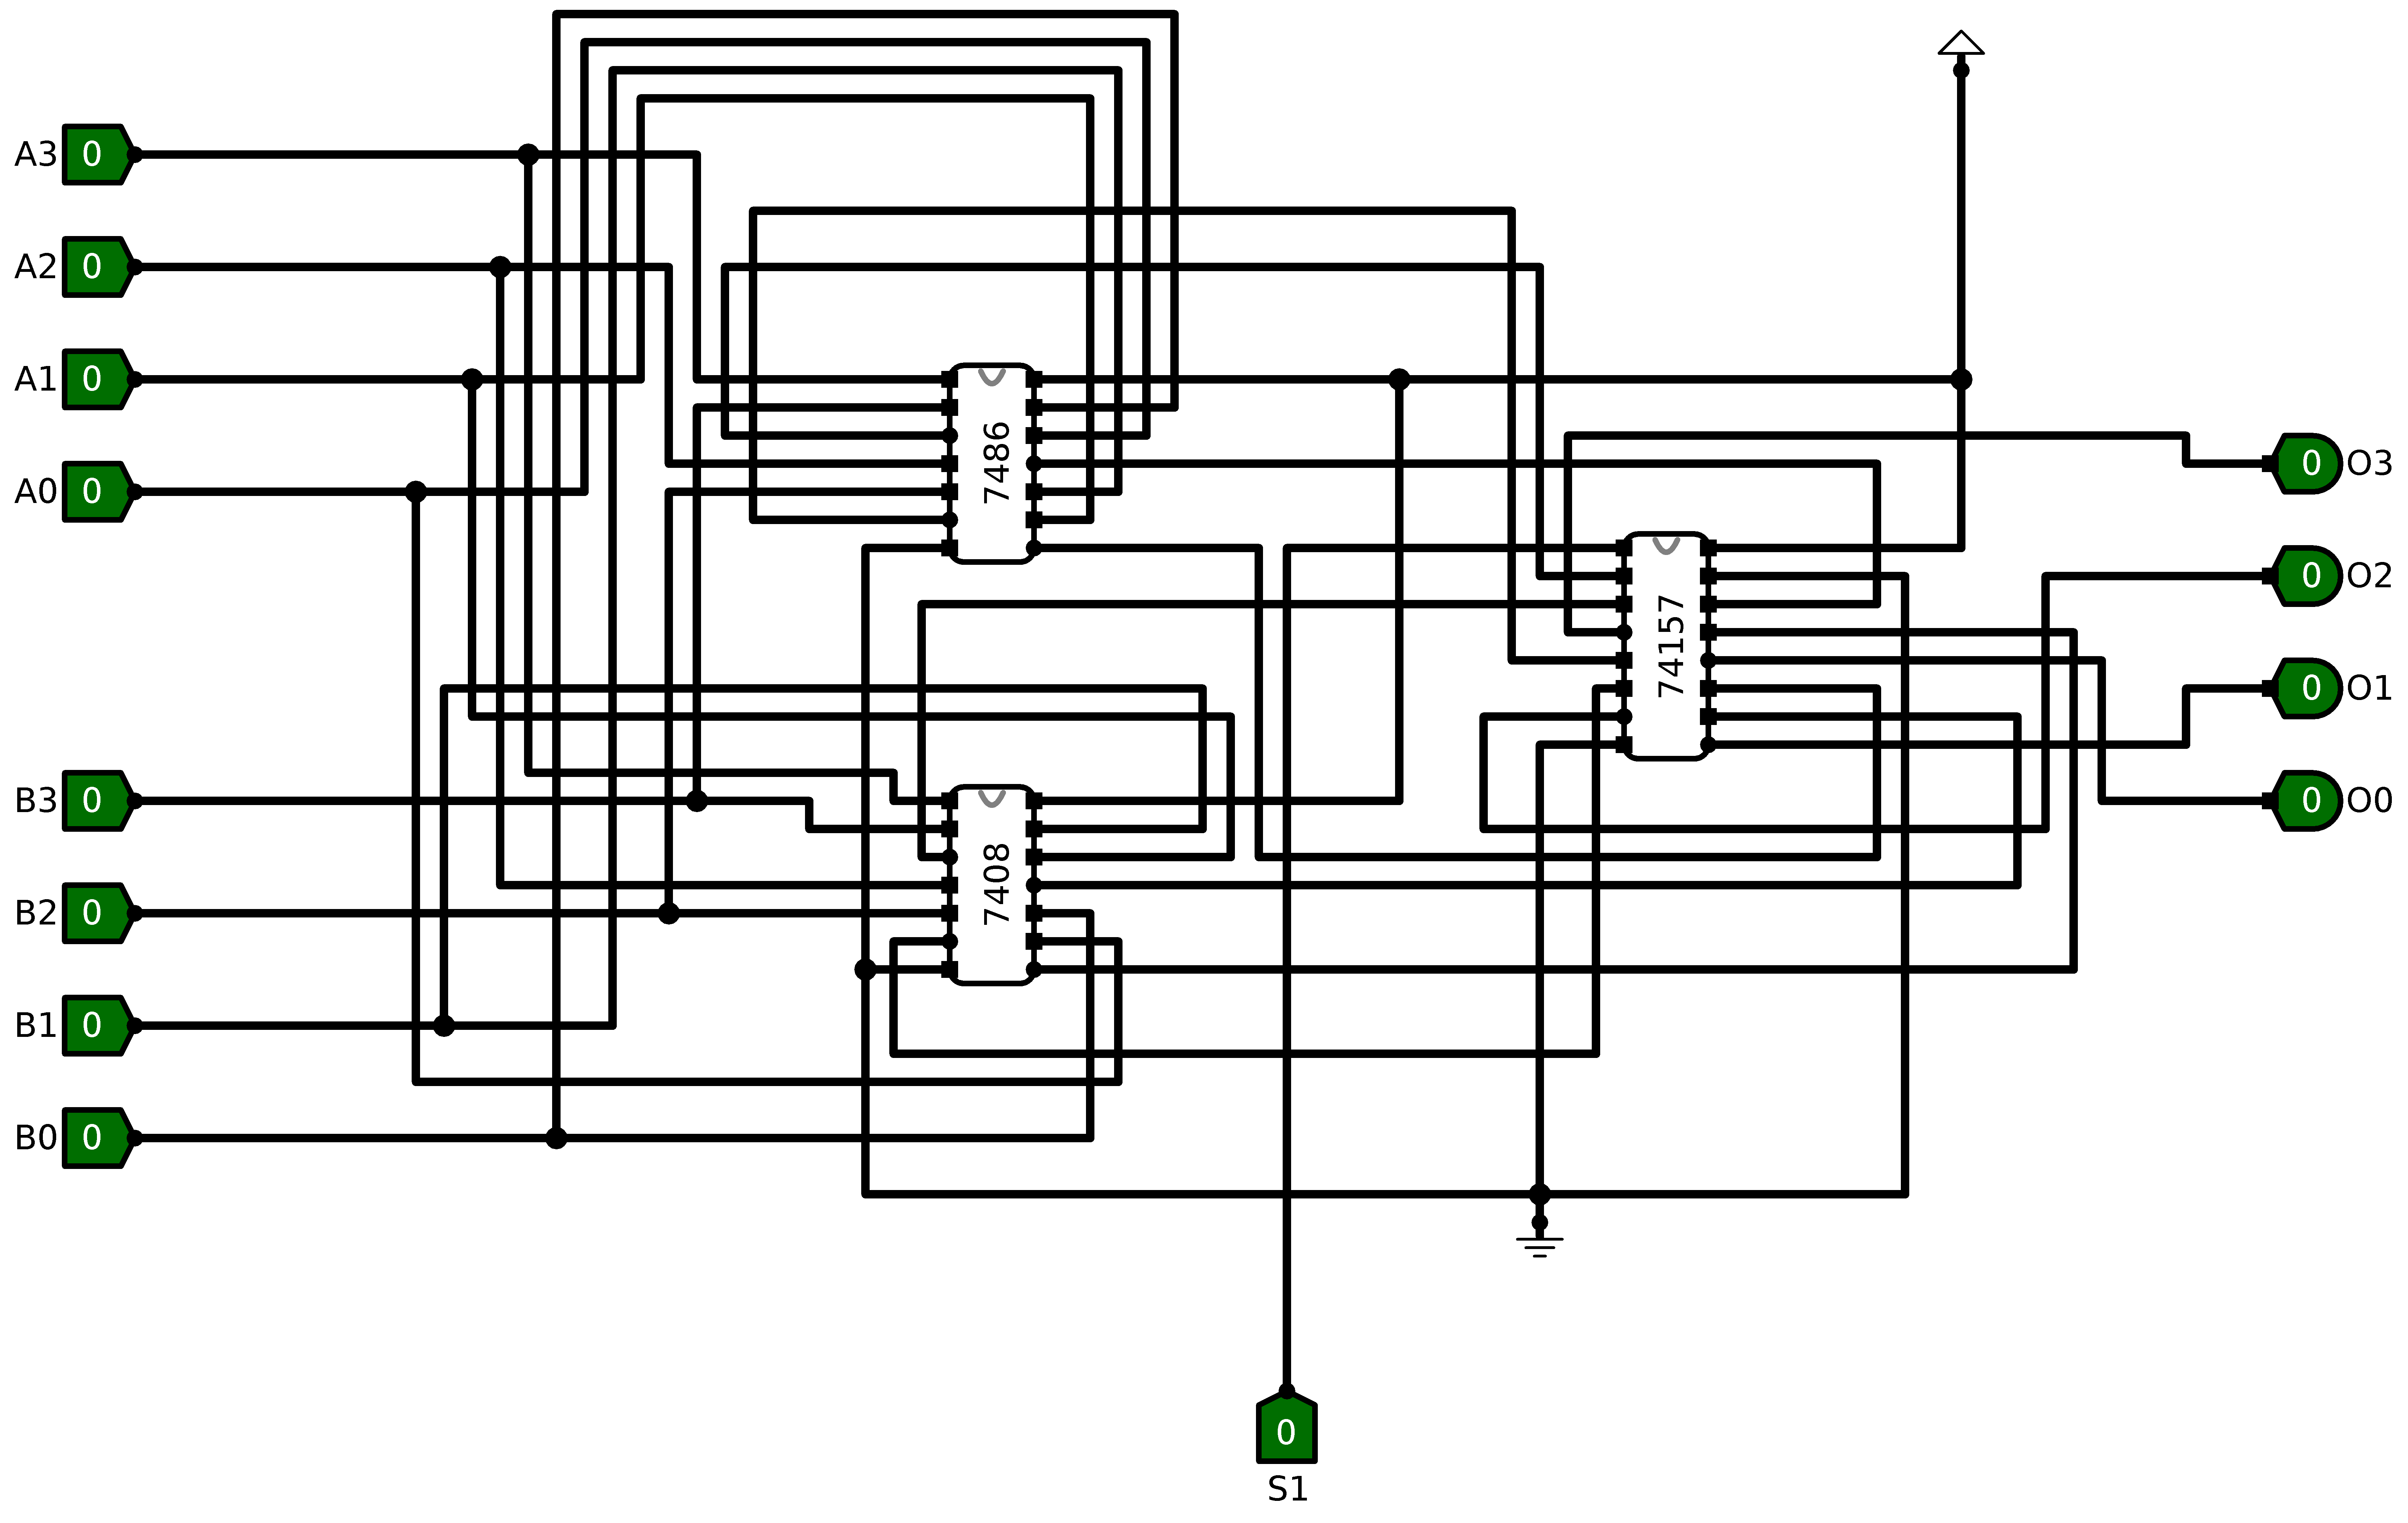
\includegraphics[width=0.8\textwidth]{Logic Unit.png}
         \caption{Logic Unit}
         \label{fig:alu_c}
     \end{figure}
     \begin{figure}[H]
         \centering
         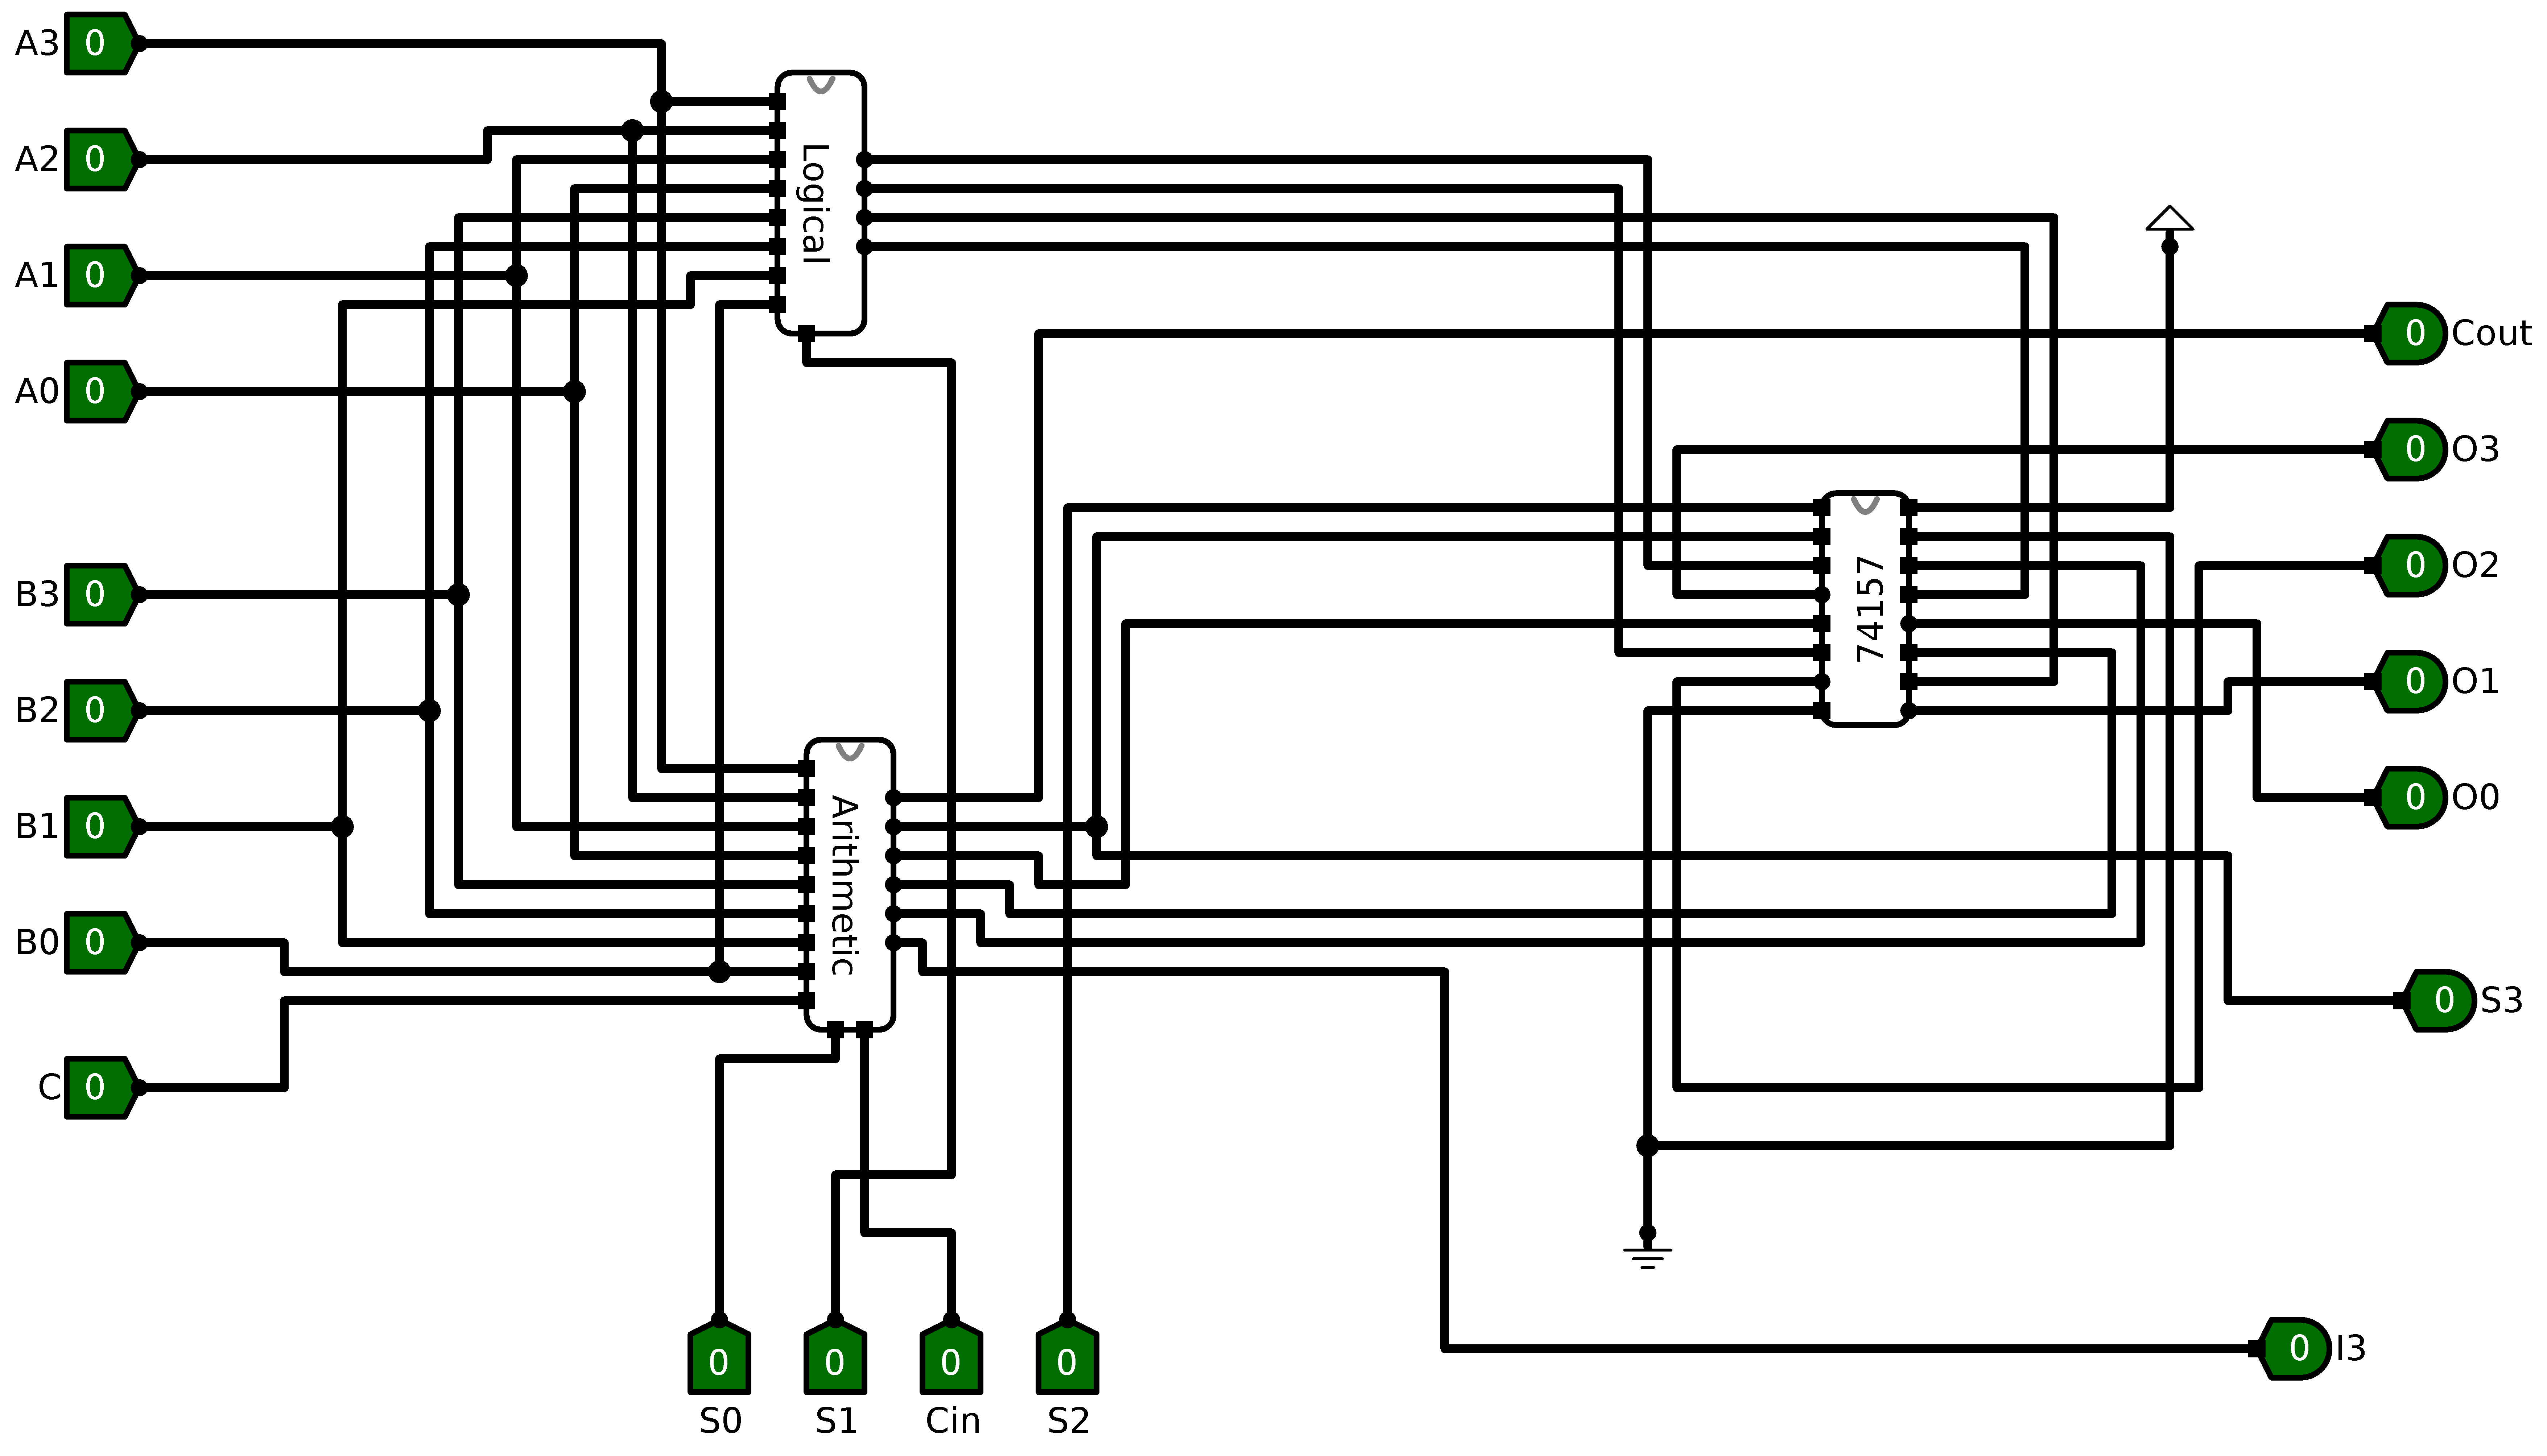
\includegraphics[width=0.8\textwidth]{Combined1.png}
         \caption{Multiplexed Arithmetic and Logic Unit}
         \label{fig:alu_d}
     \end{figure}

     \begin{figure}[H]
         \centering
         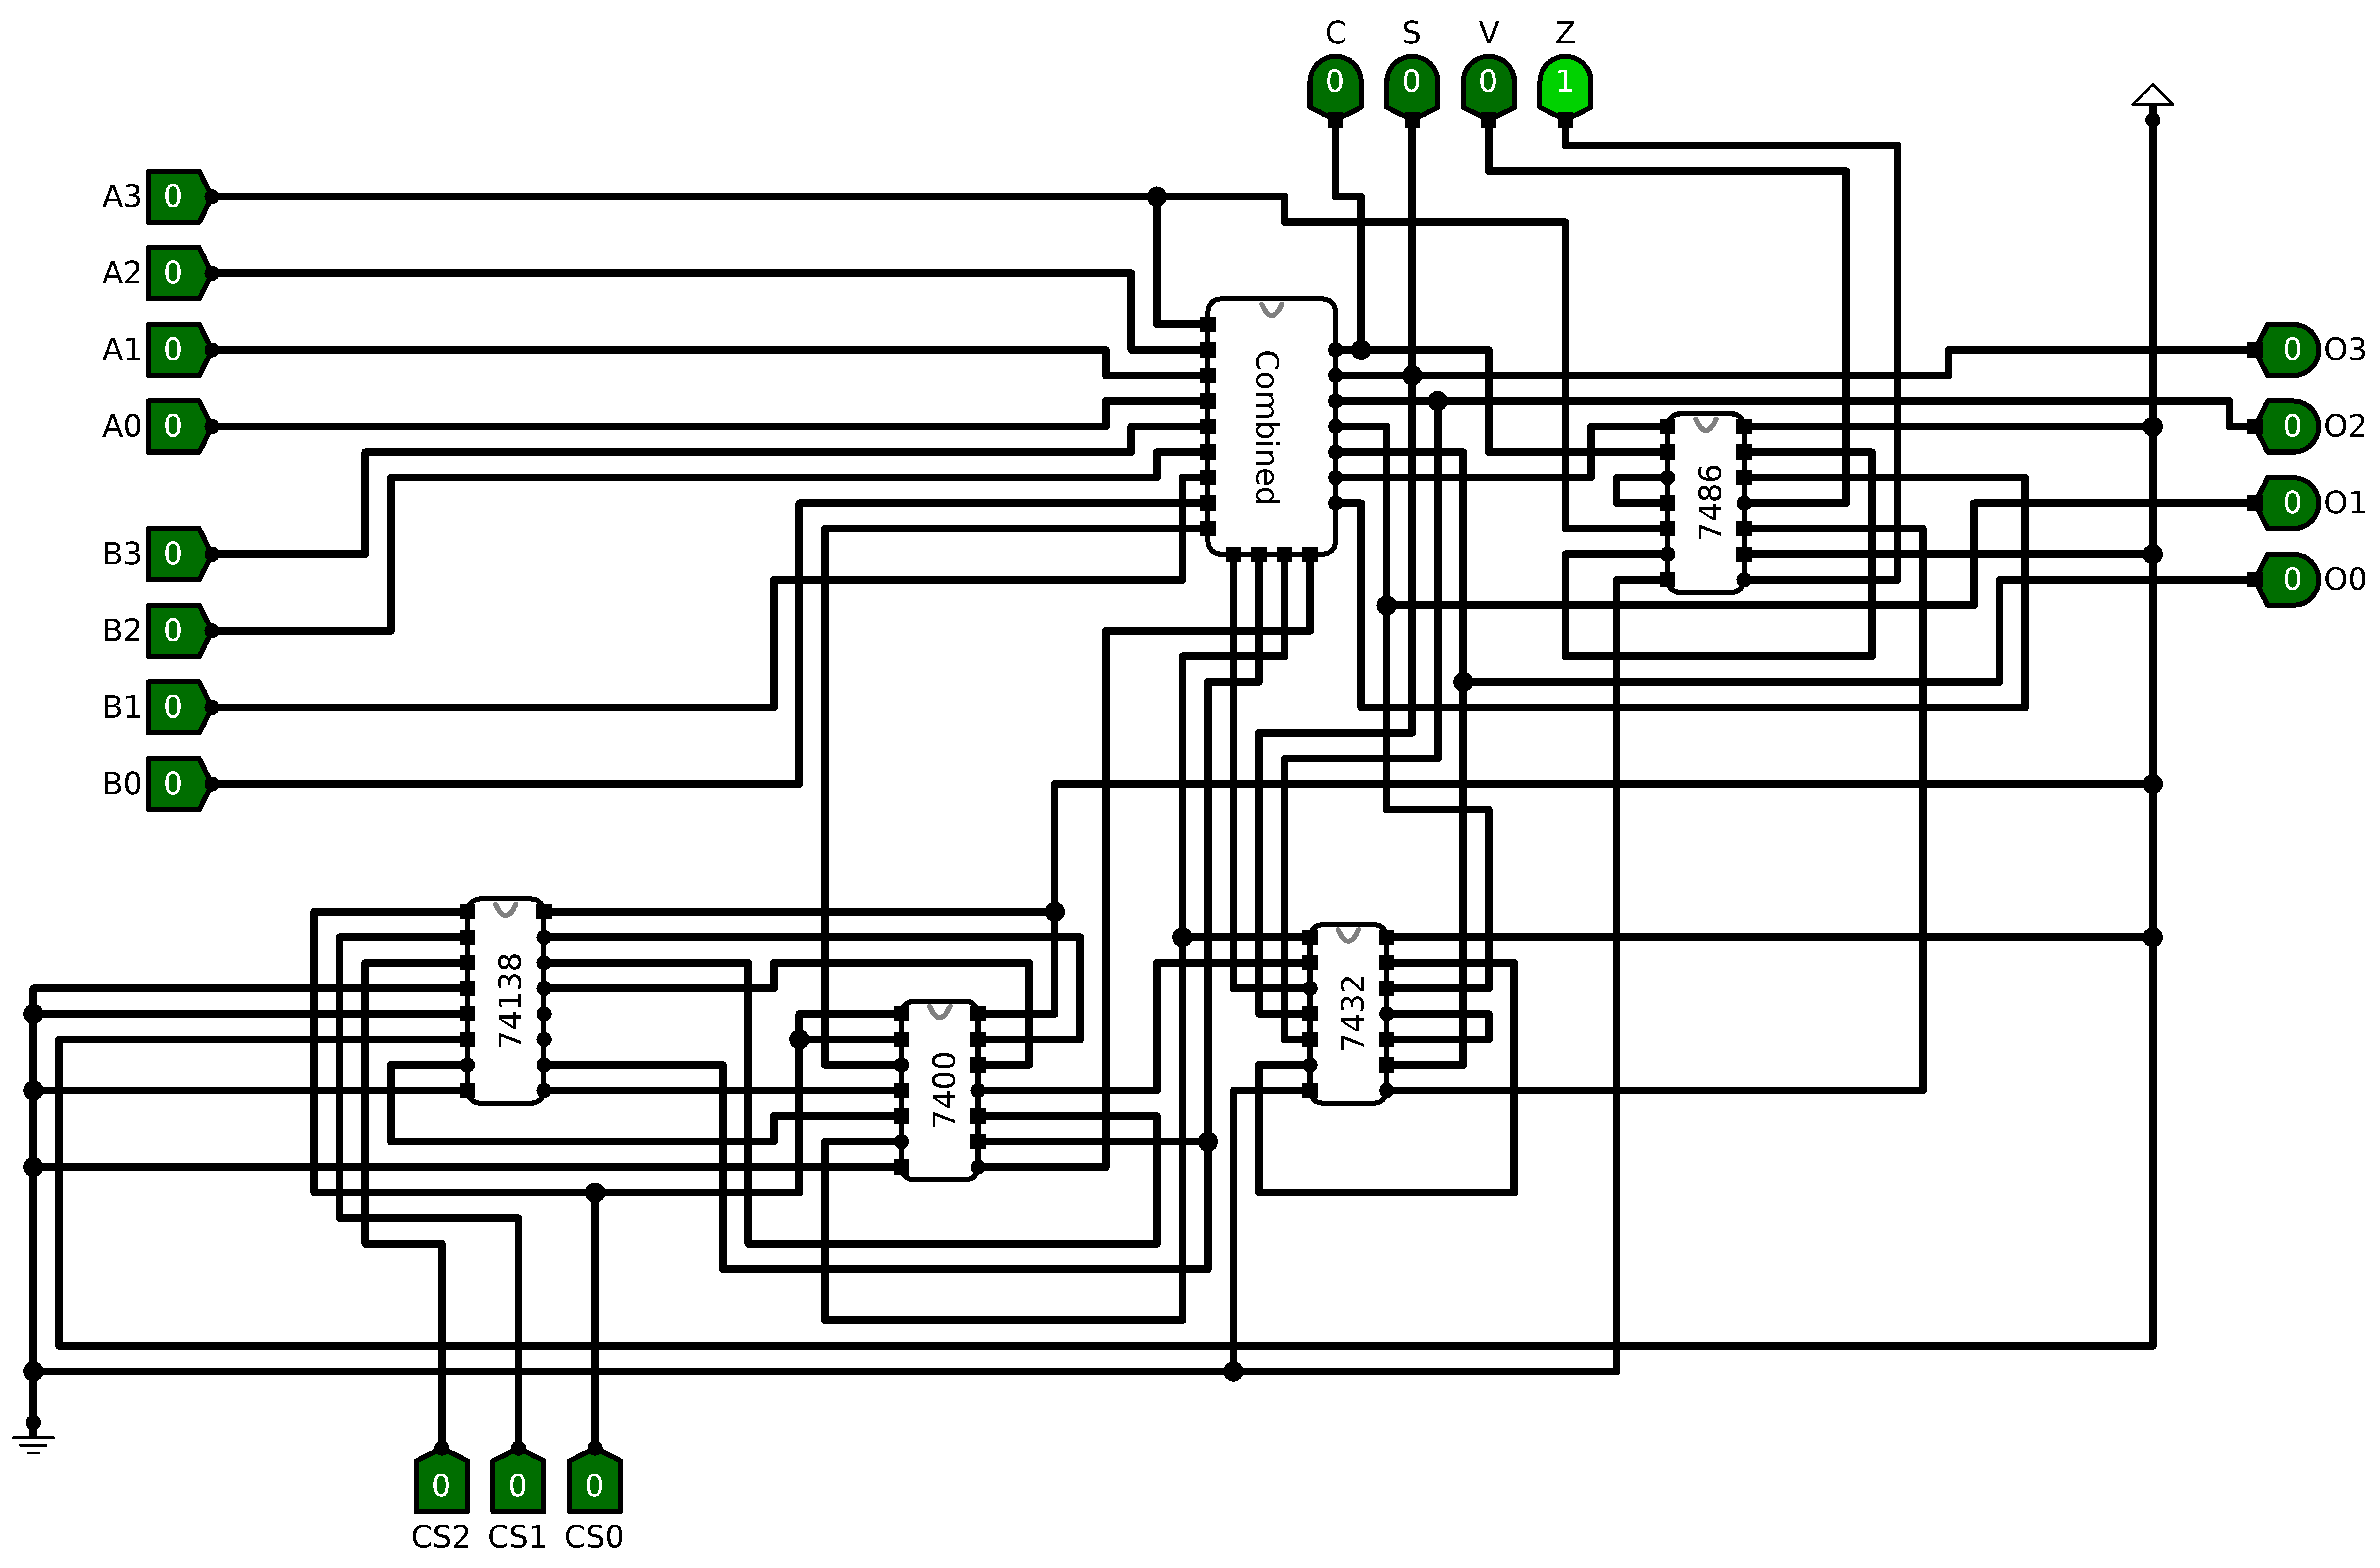
\includegraphics[width=0.7\textwidth]{ALU.png}
         \caption{The ALU}
         \label{fig:alu_e}
     \end{figure}



\begin{figure}[H]
    \centering
    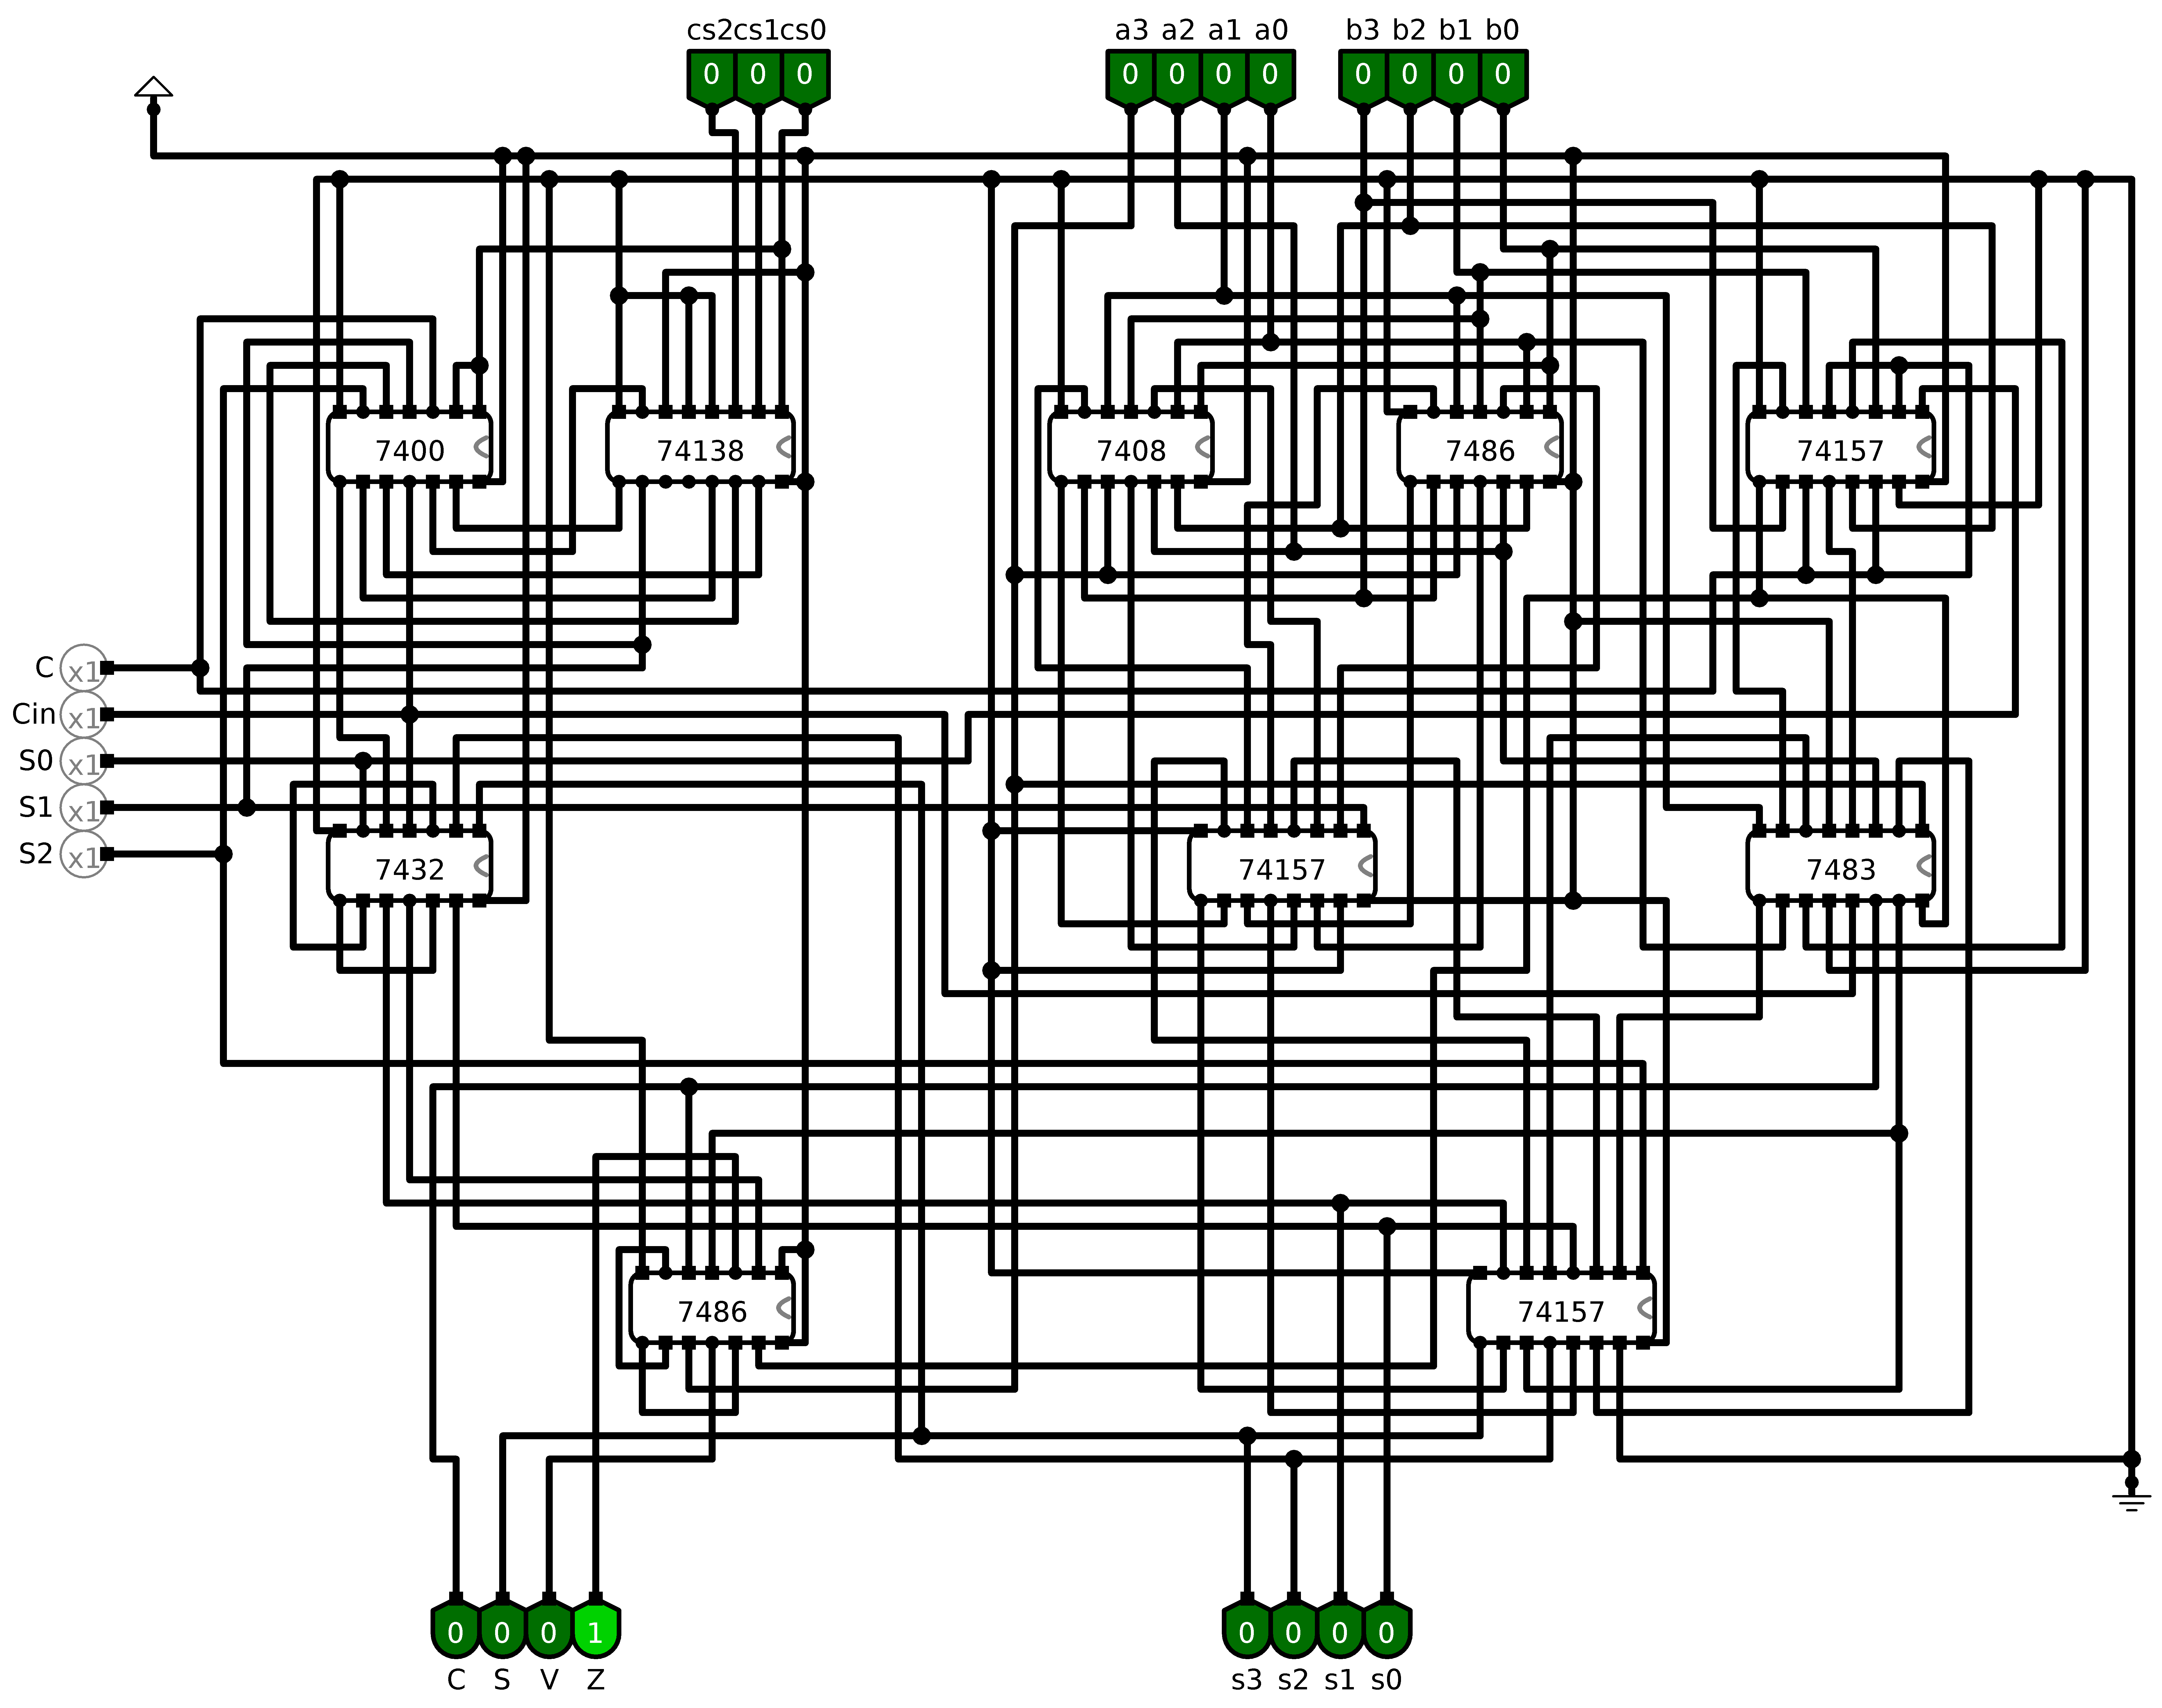
\includegraphics[width=0.8\textwidth]{combined.png}
    \caption{The Complete Design}
    \label{fig:comb}
\end{figure}

\newpage
\section{\large{ICs Used with Count as a Chart}}
\begin{table}[H]
    \centering
    \begin{tabular}{lc}
         \textbf{IC} & \textbf{Quantity}  \\
         \hline
         \hline
         IC 7400 & 1  \\
         IC 7408 & 1  \\
         IC 7432 & 1  \\
         IC 7483 & 1  \\
         IC 7486 & 2  \\
         IC 74138 & 1  \\
         IC 74157 & 3  \\
         \hline
         Total & 10  \\
    \end{tabular}
    \caption{ICs Used with Quantity}
    \label{tab:ic_quantity}
\end{table}


\newpage
\section{\large{The Simulator Used along with the Version Number}}
Logisim - 2.7.1

\section{\large{Discussion}}
In this assignment, we were tasked to implement a $4$-bit ALU which performs $4$ arithmetic and $2$ logical operations.\\
Through rigorous scrutiny, we had to strive hard to obtain the design with the minimum number of ICs. In achieving this, we had to make optimizations like performing the logical NOT operation with IC$7486$ (XOR) or manipulating one of the IC$7483$ (Adder) inputs to achieve various arithmetic operations. They were results of multiple runs of redoing the design.\\
The hardware implementation also posed challenges like planning the placement of different modules. To keep the hardware design clean, we had to connect the wires so that they cross as little length as possible between the connections. Extra effort had to be invested to make the hardware not just working, but aesthetically pleasing. Power and ground connection were done with caution to prevent IC or other components from getting damaged. \\
After checking all the boxes, we are hopefully successful in implementing the $4$-bit Arithmetic and Logic Unit (ALU) with minimum number of ICs.
\end{document}
